\subsection{Amélioration de la factorisation et de la résolution triangulaire}
Dans un premier temps, nous allons nous consacrer sur l'amélioration de la parallélisation de la factorisation ILU(k).
%
Chaque tâche du DAG représente la factorisation d'une ligne de la matrice.
%
Cette granularité est trop fine, mais c'est voulu, elle représente la granularité que nous obtenons en décrivant naturellement le maximum  de parallélisme que nous pouvons exploiter.
%
Nous avons factorisé 4 matrices différentes, il y a un cube généré de taille 80 éléments de côté avec des éléments de taille différents (1, 3, 8), il y a aussi la matrice qui représente le cas test SPE10 qui a des éléments de taille 3.
%
Les résultats obtenus avec des cubes générés de tailles différentes sont équivalent au cube de taille 80.
%
Comme le montre la figure~\ref{fig:res_facto_no_agg}, la taille des éléments a une importance considérable sur les performances que nous obtenons.
%
L'utilisation de 2 threads n'est viable que dans le cas où les éléments ont une taille de 8.
%
Dans les autres cas, même en utilisant 4 threads, nous perdons du temps.
%
Ici, la taille des éléments va définir le nombre d'opérations faites par ligne de la matrice, donc plus cette taille est grande, plus il y aura de travail à faire.
%
Ces résultats confirment notre problème de granularité.
%
Au final, avec l'utilisation des 12 coeurs de calcul de la machine, nous obtenons des speedup plutôt décevant, par exemple, pour des éléments de taille 3, le code tourne environ 2,5x plus vite que la version séquentielle mais il utilise 12 threads.


%   (-_-)   %
\begin{figure}[t!]
  \centering
  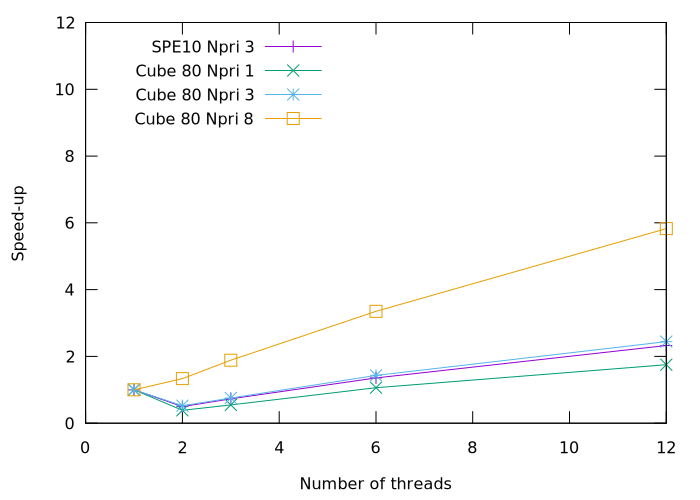
\includegraphics[width=0.7\textwidth]{res_facto_no_agg}
  \caption{Performance de la factorisation sur 12 coeurs sans utiliser Taggre.}
  \label{fig:res_facto_no_agg}
\end{figure}

Dans un premier temps, nous allons applique l'opérateur F avec le paramètre 36.
%
Cet opérateur va donc limiter la largeur du graphe pour qu'il y est au plus 36 tâches par hauteur du graphe.
%
Nous réduisons donc le parallélisme mais nous réduisons aussi le nombre de tâches, on divise par 62 le nombre de tâches pour un cube de 80 de côté.
%
La figure~\ref{fig:res_facto_f36} nous montre une amélioration du temps de factorisation quand le nombre de variables primaires est faible, le surcoût d'ordonnancement de la tâche est du même ordre de grandeur que le temps de calcul de la tâche.
%
Dans le cas où le nombre de variables primaires est élevé, il n'y a pas beaucoup d'amélioration.


%   (-_-)   %
\begin{figure}[t!]
  \centering
  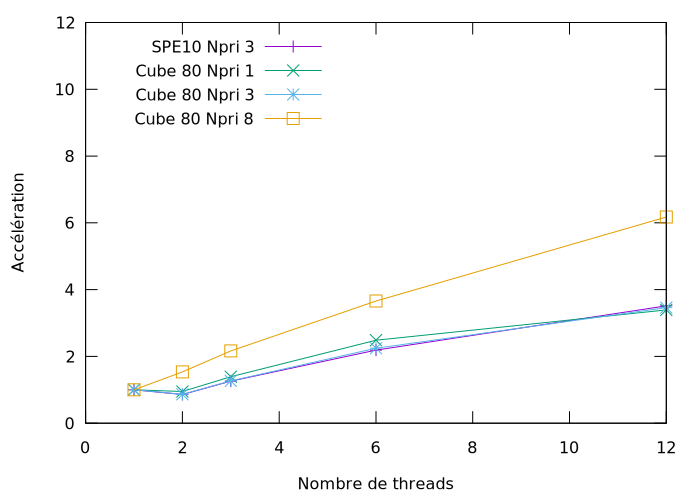
\includegraphics[width=0.7\textwidth]{res_facto_f36}
  \caption{Performance de la factorisation sur 12 coeurs avec Taggre F(36).}
  \label{fig:res_facto_f36}
\end{figure}

Essayons maintenant l'opérateur D avec le paramètre 8.
%
Cet opérateur va essayer de créer des groupes de 8 tâches assez proches dans le graphe.
%
Nous allons donc diviser par 8 le nombre de tâches, ce qui peut paraître peu mais cette valeur a été choisie empiriquement parmi un ensemble de valeur.
%
Comparé à l'opérateur F, il y a très peu d'amélioration quand le nombre de variables primaires est faible (Fig.~\ref{fig:res_facto_d8}).
%
Par contre, avec 8 variables primaires, on obtient un gain de performance qui est dû à une meilleure utilisation des caches, surtout du cache L2 avec une diminution de 10\% des défauts de cache.

%   (-_-)   %
\begin{figure}[t!]
  \centering
  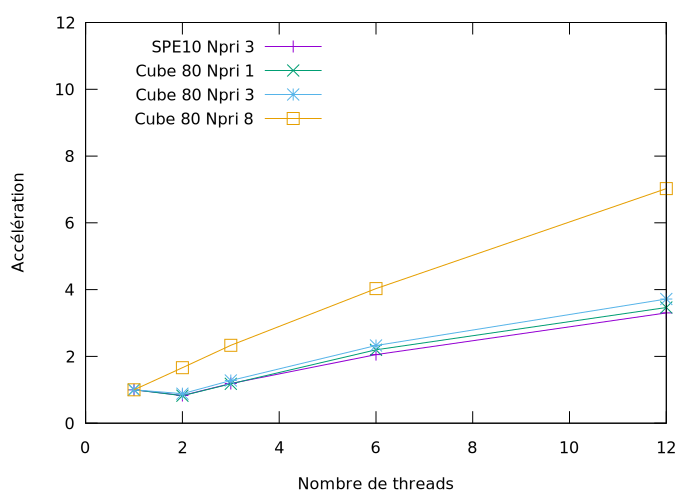
\includegraphics[width=0.7\textwidth]{res_facto_d8}
  \caption{Performance de la factorisation sur 12 coeurs avec Taggre D(8).}
  \label{fig:res_facto_d8}
\end{figure}

Les deux précèdent opérateurs donnent déjà des résultats, mais le meilleur opérateur pour nos matrices reste l'opérateur C.
%
Comme le montre les résultats de la figure~\ref{fig:res_facto_c}, tous les cas tests sont améliorés.
%
Il y a deux grandes améliorations, comme pour tous les opérateurs, il y a une réduction du nombre de tâches, mais dans ce cas la réduction est bien plus importante.
%
En effet, avec l'opérateur F, le nombre de tâches était fortement réduit mais les tâches agrégés n'avaient pas une bonne réutilisabilité des données en cache.
%
Au contraire, l'opérateur D ne réduisait que de très peu le donc de tâches mais améliorait la réutilisation des caches.
%
L'opérateur C offre le meilleur des deux opérateurs, il produit peu de tâches et en plus ces tâches réutilisent correctement les données en cache.
% L2 stats : F:1.10, D:0.96, C:0.87


%   (-_-)   %
\begin{figure}[t!]
  \centering
  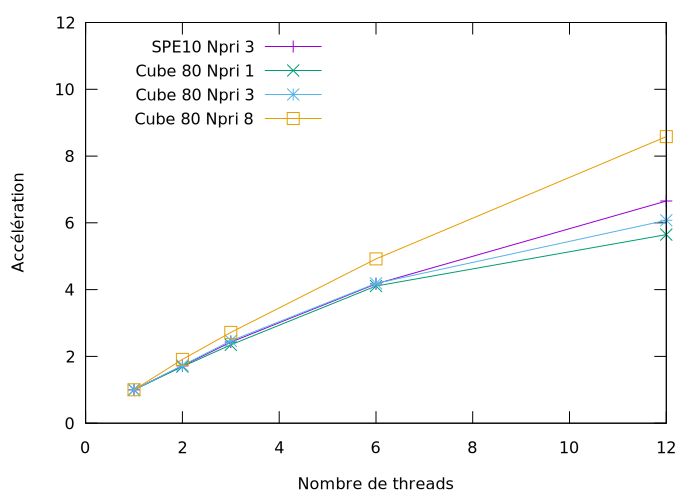
\includegraphics[width=0.7\textwidth]{res_facto_c}
  \caption{Performance de la factorisation sur 12 coeurs avec Taggre C.}
  \label{fig:res_facto_c}
\end{figure}

Il est aussi possible de combiner plusieurs opérateurs, sur la figure~\ref{fig:res_facto_cd2} nous avons combiné l'opérateur C avec l'opérateur D(2).
%
On observe un très léger gain de performance qu'en on a une seule variable primaire, mais dans les autres cas on observe le contraire.
%
Malgré ces optimisations, nous n'atteignons pas un speedup parfait, avec au mieux 8,7 de speedup pour 12 coeurs.
%
Nous expliquerons ce souci de performance dans les parties suivantes de la thèse.

%   (-_-)   %
\begin{figure}[t!]
  \centering
  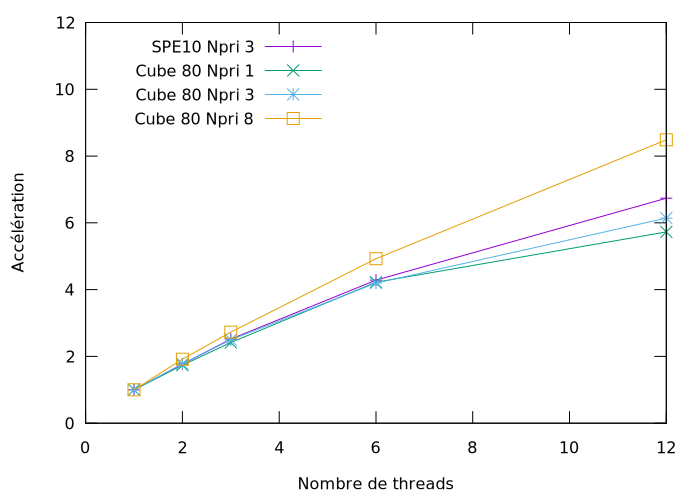
\includegraphics[width=0.7\textwidth]{res_facto_cd2}
  \caption{Performance de la factorisation sur 12 coeurs avec Taggre CD(2).}
  \label{fig:res_facto_cd2}
\end{figure}

Essayons maintenant cette technique sur la partie résolution triangulaire du code.
%
Les performances sans agrégations sont bien en dessous de la partie factorisation (Fig.\ref{fig:res_trsv_no_agg}).
%
Même en utilisant 12 threads, seule la version avec 8 variables primaires donne de meilleurs résultats que la version séquentielle.
%
Encore une fois il s'agit d'un problème de granularité, le graphe à ordonnancer est le même que pour la factorisation mais les tâches sont plus petites.
%
Si nous regardons les résultats avec la meilleure agrégation que nous ayons, l'agrégation CD(2), on obtient des résultats légèrement meilleurs mais on n'est encore loin du speedup parfait.

%   (-_-)   %
\begin{figure}[t!]
  \centering
  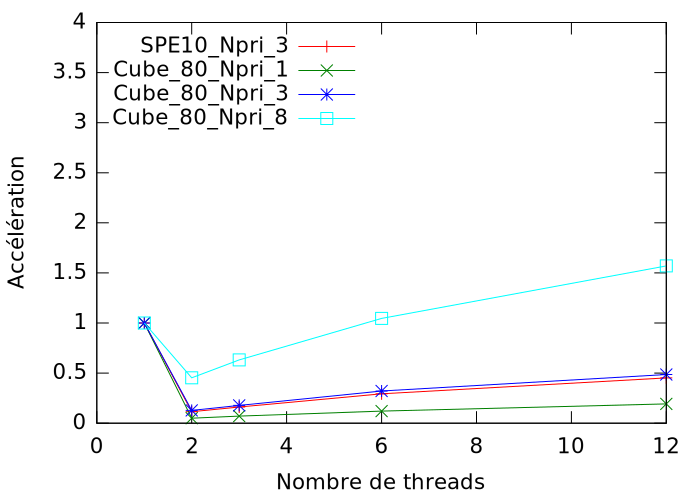
\includegraphics[width=0.7\textwidth]{res_trsv_no_agg}
  \caption{Performance de la résolution triangulaire sur 12 coeurs sans utiliser Taggre.}
  \label{fig:res_trsv_no_agg}
\end{figure}


%   (-_-)   %
\begin{figure}[t!]
  \centering
  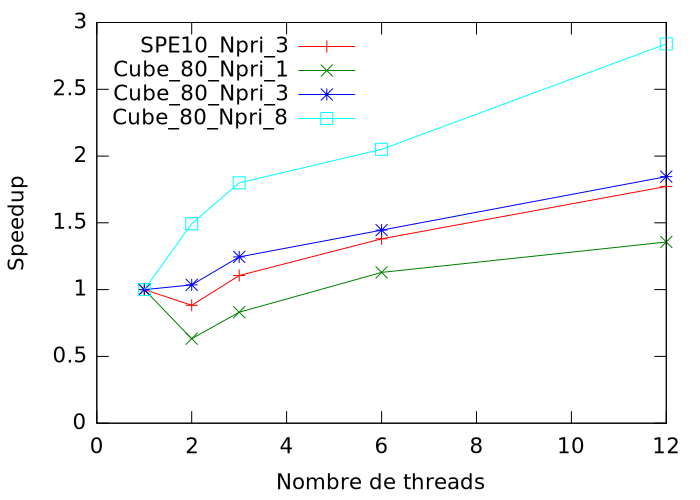
\includegraphics[width=0.7\textwidth]{res_trsv_cd2}
  \caption{Performance de la résolution triangulaire sur 12 coeurs sans utiliser Taggre.}
  \label{fig:res_trsv_cd2}
\end{figure}

%% +---------------------------+-------------+-------------+-------------+------------+
%% |          Metric           |     Sum     |     Max     |     Min     |    Avg     |
%% +---------------------------+-------------+-------------+-------------+------------+
%% | Runtime (RDTSC) [s] STAT  |   1923.94   |   160.328   |   160.328   |  160.328   |
%% | Runtime unhalted [s] STAT |   1870.36   |   160.82    |   152.347   |  155.864   |
%% |     Clock [MHz] STAT      |   34528.4   |   2906.13   |   2850.24   |  2877.37   |
%% |         CPI STAT          |   1.03608   |   1.04174   |   1.02468   | 0.0863398  |
%% |  Data cache misses STAT   | 4.59444e+10 | 4.08753e+09 | 3.71715e+09 | 3.8287e+09 |
%% | Data cache miss rate STAT |   0.10934   | 0.00932521  | 0.00905509  | 0.0091117  |
%% +---------------------------+-------------+-------------+-------------+------------+
%% +---------------------------+-------------+-------------+-------------+-------------+
%% |          Metric           |     Sum     |     Max     |     Min     |     Avg     |
%% +---------------------------+-------------+-------------+-------------+-------------+
%% | Runtime (RDTSC) [s] STAT  |   2004.24   |   167.02    |   167.02    |   167.02    |
%% | Runtime unhalted [s] STAT |   2061.97   |   175.567   |   170.297   |   171.831   |
%% |     Clock [MHz] STAT      |   36151.6   |   3017.39   |   3008.02   |   3012.64   |
%% |         CPI STAT          |   1.14231   |   1.14711   |   1.13205   |  0.0951929  |
%% |  Data cache misses STAT   | 4.87067e+10 | 4.29088e+09 | 4.00937e+09 | 4.05889e+09 |
%% | Data cache miss rate STAT |  0.115926   | 0.00990628  | 0.00962271  | 0.00966052  |
%% +---------------------------+-------------+-------------+-------------+-------------+
%% +---------------------------+-------------+-------------+-------------+-------------+
%% |          Metric           |     Sum     |     Max     |     Min     |     Avg     |
%% +---------------------------+-------------+-------------+-------------+-------------+
%% | Runtime (RDTSC) [s] STAT  |   1640.85   |   136.737   |   136.737   |   136.737   |
%% | Runtime unhalted [s] STAT |   1686.77   |   144.388   |   138.353   |   140.564   |
%% |     Clock [MHz] STAT      |   36255.7   |   3046.34   |   2998.08   |   3021.31   |
%% |         CPI STAT          |  0.934931   |  0.937527   |  0.926718   |  0.0779109  |
%% |  Data cache misses STAT   | 3.85951e+10 | 3.43628e+09 | 3.14135e+09 | 3.21626e+09 |
%% | Data cache miss rate STAT |  0.0919074  | 0.00789712  | 0.00762214  | 0.00765895  |
%% +---------------------------+-------------+-------------+-------------+-------------+




%% +---------------------------+----------+-----------+-----------+-----------+
%% |          Metric           |   Sum    |    Max    |    Min    |    Avg    |
%% +---------------------------+----------+-----------+-----------+-----------+
%% | Runtime (RDTSC) [s] STAT  | 2013.52  |  167.794  |  167.794  |  167.794  |
%% | Runtime unhalted [s] STAT |  2049.5  |  173.386  |  167.781  |  170.792  |
%% |     Clock [MHz] STAT      | 35861.8  |  3005.94  |  2972.33  |  2988.48  |
%% |         CPI STAT          | 1.13698  |  1.14624  |  1.12814  | 0.0947487 |
%% |   L2 request rate STAT    | 0.139712 | 0.0119216 | 0.0115742 | 0.0116426 |
%% |     L2 miss rate STAT     | 0.154052 | 0.0129583 | 0.0127815 | 0.0128376 |
%% |    L2 miss ratio STAT     | 13.2323  |  1.10948  |  1.08696  |  1.10269  |
%% +---------------------------+----------+-----------+-----------+-----------+
%% +---------------------------+----------+-----------+-----------+-----------+
%% |          Metric           |   Sum    |    Max    |    Min    |    Avg    |
%% +---------------------------+----------+-----------+-----------+-----------+
%% | Runtime (RDTSC) [s] STAT  | 1966.96  |  163.913  |  163.913  |  163.913  |
%% | Runtime unhalted [s] STAT | 1886.06  |  158.261  |  156.494  |  157.172  |
%% |     Clock [MHz] STAT      | 34326.8  |  2883.42  |  2837.74  |  2860.57  |
%% |         CPI STAT          | 1.03718  |  1.06006  |  1.01601  | 0.0864318 |
%% |   L2 request rate STAT    | 0.152488 | 0.0130698 | 0.0125945 | 0.0127073 |
%% |     L2 miss rate STAT     | 0.14729  | 0.0125144 | 0.0121436 | 0.0122742 |
%% |    L2 miss ratio STAT     | 11.5912  | 0.970545  | 0.957504  | 0.965933  |
%% +---------------------------+----------+-----------+-----------+-----------+
%% +---------------------------+----------+-----------+-----------+-----------+
%% |          Metric           |   Sum    |    Max    |    Min    |    Avg    |
%% +---------------------------+----------+-----------+-----------+-----------+
%% | Runtime (RDTSC) [s] STAT  |  1652.6  |  137.716  |  137.716  |  137.716  |
%% | Runtime unhalted [s] STAT | 1694.79  |  142.824  |  140.196  |  141.233  |
%% |     Clock [MHz] STAT      | 36166.7  |  3035.99  |  2993.16  |  3013.9   |
%% |         CPI STAT          | 0.937105 | 0.962554  | 0.921956  | 0.0780921 |
%% |   L2 request rate STAT    | 0.158081 | 0.0134666 | 0.0131121 | 0.0131734 |
%% |     L2 miss rate STAT     | 0.138087 | 0.0116948 | 0.0114514 | 0.0115072 |
%% |    L2 miss ratio STAT     | 10.4823  |  0.87775  |  0.86843  | 0.873526  |
%% +---------------------------+----------+-----------+-----------+-----------+


%% +---------------------------+----------+-----------+---------+------------+
%% |          Metric           |   Sum    |    Max    |   Min   |    Avg     |
%% +---------------------------+----------+-----------+---------+------------+
%% | Runtime (RDTSC) [s] STAT  | 2014.07  |  167.839  | 167.839 |  167.839   |
%% | Runtime unhalted [s] STAT | 2045.66  |  172.625  | 168.205 |  170.471   |
%% |     Clock [MHz] STAT      | 35826.2  |  3000.16  | 2971.72 |  2985.52   |
%% |         CPI STAT          | 1.13743  |  1.14473  | 1.12957 | 0.0947856  |
%% |   L3 request rate STAT    | 0.085237 | 0.0429422 |    0    | 0.00710308 |
%% |     L3 miss rate STAT     | 0.116483 | 0.0586274 |    0    | 0.00970692 |
%% |    L3 miss ratio STAT     |  1.1549  | 0.577687  |    0    | 0.0962418  |
%% +---------------------------+----------+-----------+---------+------------+
%% +---------------------------+-----------+-----------+---------+------------+
%% |          Metric           |    Sum    |    Max    |   Min   |    Avg     |
%% +---------------------------+-----------+-----------+---------+------------+
%% | Runtime (RDTSC) [s] STAT  |  1932.6   |  161.05   | 161.05  |   161.05   |
%% | Runtime unhalted [s] STAT |  1869.75  |  159.171  | 152.621 |  155.813   |
%% |     Clock [MHz] STAT      |  34423.7  |  2896.06  | 2841.43 |  2868.64   |
%% |         CPI STAT          |  1.03599  |  1.03868  | 1.03237 | 0.0863323  |
%% |   L3 request rate STAT    | 0.0858767 | 0.0432998 |    0    | 0.00715639 |
%% |     L3 miss rate STAT     | 0.106569  | 0.0534681 |    0    | 0.00888075 |
%% |    L3 miss ratio STAT     |  1.10754  | 0.554997  |    0    | 0.0922947  |
%% +---------------------------+-----------+-----------+---------+------------+
%% +---------------------------+-----------+-----------+----------+------------+
%% |          Metric           |    Sum    |    Max    |   Min    |    Avg     |
%% +---------------------------+-----------+-----------+----------+------------+
%% | Runtime (RDTSC) [s] STAT  |  1696.46  |  141.372  | 141.372  |  141.372   |
%% | Runtime unhalted [s] STAT |  1699.84  |  146.474  | 137.316  |  141.654   |
%% |     Clock [MHz] STAT      |  35865.4  |  3011.87  | 2965.87  |  2988.79   |
%% |         CPI STAT          | 0.931982  | 0.946119  | 0.924821 | 0.0776651  |
%% |   L3 request rate STAT    | 0.0785352 | 0.0400494 |    0     | 0.0065446  |
%% |     L3 miss rate STAT     | 0.0962549 | 0.0481313 |    0     | 0.00802125 |
%% |    L3 miss ratio STAT     |  1.10147  |  0.55564  |    0     | 0.0917888  |
%% +---------------------------+-----------+-----------+----------+------------+



%% +---------------------------------+------------+-------------+-------------+-------------+
%% |             Metric              |    Sum     |     Max     |     Min     |     Avg     |
%% +---------------------------------+------------+-------------+-------------+-------------+
%% |    Runtime (RDTSC) [s] STAT     |  2070.55   |   172.546   |   172.546   |   172.546   |
%% |    Runtime unhalted [s] STAT    |  2068.93   |   175.779   |   169.669   |   172.411   |
%% |        Clock [MHz] STAT         |  35538.6   |   3007.39   |   2915.92   |   2961.55   |
%% |            CPI STAT             |  1.13513   |   1.15526   |   1.11284   |  0.094594   |
%% |        Branch rate STAT         |  0.905246  |  0.0790124  |  0.0746446  |  0.0754372  |
%% | Branch misprediction rate STAT  | 0.00516248 | 0.000476814 | 0.000405921 | 0.000430207 |
%% | Branch misprediction ratio STAT | 0.0684119  | 0.00618842  | 0.00543805  | 0.00570099  |
%% |  Instructions per branch STAT   |  159.109   |   13.3968   |   12.6562   |   13.2591   |
%% +---------------------------------+------------+-------------+-------------+-------------+

%% +---------------------------------+------------+-------------+-------------+-------------+
%% |             Metric              |    Sum     |     Max     |     Min     |     Avg     |
%% +---------------------------------+------------+-------------+-------------+-------------+
%% |    Runtime (RDTSC) [s] STAT     |  1961.67   |   163.472   |   163.472   |   163.472   |
%% |    Runtime unhalted [s] STAT    |  1876.49   |   158.39    |   154.522   |   156.374   |
%% |        Clock [MHz] STAT         |  34367.1   |   2882.84   |   2844.95   |   2863.92   |
%% |            CPI STAT             |   1.0338   |   1.05326   |   1.01697   |  0.0861503  |
%% |        Branch rate STAT         |  0.897154  |  0.0761396  |  0.0736554  |  0.0747628  |
%% | Branch misprediction rate STAT  | 0.00511161 | 0.000463287 | 0.000395029 | 0.000425968 |
%% | Branch misprediction ratio STAT | 0.0683374  | 0.00613752  | 0.00536154  | 0.00569478  |
%% |  Instructions per branch STAT   |  160.529   |   13.5767   |   13.1338   |   13.3774   |
%% +---------------------------------+------------+-------------+-------------+-------------+






%% +---------------------------+---------+---------+---------+-----------+
%% |          Metric           |   Sum   |   Max   |   Min   |    Avg    |
%% +---------------------------+---------+---------+---------+-----------+
%% | Runtime (RDTSC) [s] STAT  | 1961.79 | 163.482 | 163.482 |  163.482  |
%% | Runtime unhalted [s] STAT | 1874.13 | 160.463 | 152.47  |  156.177  |
%% |     Clock [MHz] STAT      | 34317.2 | 2879.83 | 2839.8  |  2859.77  |
%% |         CPI STAT          | 1.0348  | 1.05031 | 1.02074 | 0.0862334 |
%% | Load to Store ratio STAT  | 44.4467 | 3.72245 | 3.6765  |  3.70389  |
%% +---------------------------+---------+---------+---------+-----------+
